\section{PG Encoding}

\subsection{Abstract}
There is a critical need for design automation in microarchitectural
modelling and synthesis. One of the areas which lacks the necessary
automation support is synthesis of instruction codes targeting various
design optimality criteria. This paper aims to fill this gap by providing
a set of formal methods and a software tool for synthesis of instruction
codes given the description of a processor as a set of instructions.

The method is based on the Conditional Partial Order Graph (CPOG)
model introduced recently, which is a formalism for efficient specification
and synthesis of microcontrol circuits. It describes a system as a
functional composition of its behavioural scenarios, or instructions,
each of them being a partial order of events. In order to distinguish
instructions within a CPOG they are given different encodings represented
with Boolean vectors. Size and latency of the final microcontroller
significantly depends on the chosen encodings, thus efficient synthesis
of instruction codes is essential.

The paper shows that the CPOG model is a very convenient formalism
for efficient representation of processor instruction sets. It provides
a ground for a concise formulation of several encoding problems, which
are reducible to the well-known Boolean satisfiability (SAT) problem
and can be efficiently solved by modern SAT solvers. Application of
all the presented techniques is demonstrated on a processor design
example.

\subsection{Introduction}

Automated design of general purpose processing cores, application-specific
instruction-set processors (ASIPs), and distributed Systems-on-Chip
(SoCs) has gained a lot of attention from academia and industry~\cite{2006_dutt_chapter}.
New formalisms for data-path modelling are proposed~\cite{2010_mokhov_ieee}\cite{2008_sokolov_sdfs},
hardware/software co-design methodology~\cite{1993_alomary_edac}
is actively developed and applied for ASIP performance improvement,
more specific techniques (such as compiler-directed instruction set
optimisation~\cite{2002_qin_date}) are constantly introduced into
the instruction set architecture (ISA) design domain.

\begin{figure}
\begin{centering}
\vspace{-3mm}
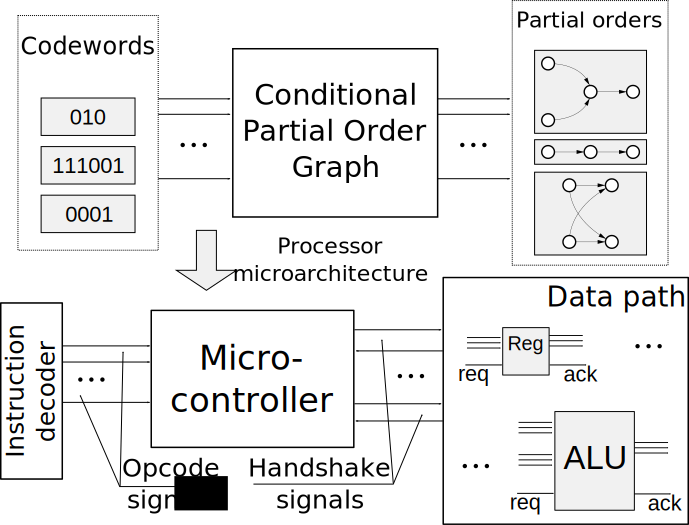
\includegraphics[width=0.6\columnwidth]{fig/control}\vspace{-1mm}

\par\end{centering}

\caption{CPOGs and processor microcontrol\label{fig:Dynamically-reconfigurable-controller}}
\vspace{-3mm}
\end{figure}


Synthesis of instruction sets is a particularly active research area.
There are methods for automated ISA synthesis for a target platform
(according to available system resources and data-path components)
and for given software requirements (e.g. aimed to ease compilation
or reduce program length). These methods eventually produce a structured
set of instructions satisfying certain properties (orthogonality,
completeness, regularity, etc.); instructions are grouped into classes
and each class is allocated a certain opcode interval within the total
code space~\cite{2003_nohl_dac}. At this point automation is typically
stopped or becomes trivial: the instructions are given arbitrary codes
within the allocated intervals. This limits performance due to instruction
decoder circuitry overheads. The problem is usually approached by
ad-hoc heuristics or application-specific optimisation techniques
(see, for example,~\cite{2002_lee_iccad}).

In this chapter we try to solve the general problem of optimal encoding
of a given set of instructions with the aid of the Conditional Partial
Order Graph (CPOG) model introduced recently~\cite{2009_mokhov_phd}\cite{2010_mokhov_ieee}.
The key features of the model are: ability to describe systems in
a compact functional form, and structural synthesis methods which
significantly improve performance of the whole design flow. These
features make the model very efficient for representation and management
of processor instruction sets in hardware and EDA software. A CPOG
is a superposition of a set of partial orders which can be extracted
from it by providing the corresponding codewords, see Figure~\ref{fig:Dynamically-reconfigurable-controller}
(top). It can be regarded as a custom associative memory for storing
cause and effect relations within a predefined set of events.

There are different kinds of systems which can be described with the
model. For example, a processor microcontroller executes partial orders
(or \textbf{instructions}) of primitive computational steps (or \textbf{microinstructions})
defined on a set of data path operational units, see Figure~\ref{fig:Dynamically-reconfigurable-controller}
(bottom). The order is determined by an \textbf{instruction}\textbf{\emph{
}}\textbf{code} --- a combination of logical conditions presented
to the controller by the environment~\cite{1994_de_micheli_book}.
To this end, the microcontroller can be seen as an entity which communicates
with two parts of the environment: one part is the source of condition
signals (an instruction decoder) and the other part is a set of controlled
objects with request-acknowledgement interface (data path operational
units which execute the microinstructions).

There are many criteria which determine the choice of a particular
processor architecture and influence design of an instruction set:
functionality, operation modes, resources, etc. In Section~\ref{sec-processor}
we study an example of an instruction set (a subset of \emph{MSP430}
processor~\cite{mspmanual}) implemented on a minimalistic hardware
platform. However, the main focus of this paper is optimal encoding
of processor instruction sets in the general architecture-independent
context. See~\cite{2011_mokhov_tr} for investigation of the architecture-level
reasoning using the CPOG model.

Main contributions of this paper are: firstly, it formulates several
instruction set encoding problems in terms of the CPOG model; secondly,
it presents the SAT characterisation of the problems leading to their
efficient automated solution; thirdly, it demonstrates application
of the CPOG methodology at different stages of a processor design
flow --- from architectural-level specification, design and behavioural
description of an instruction set to its encoding and synthesis of
the physical implementation of the microcontroller. The paper is organised
as follows. Section~\ref{sec:CPOG-model-essentials} briefly introduces
the CPOG model providing a ground for formulating a set of problems
of optimal instruction set encoding in Section~\ref{sec:Optimal-encoding-problem}.
A method for automated translation of the problems into SAT instances
is explained in Section~\ref{sec:SAT-formulation}. It is followed
by a processor design example in Section~\ref{sec-processor} and
conclusions.
